% 复数
% 矢量|虚数|复数|三角恒等式|共轭

\pentry{几何矢量\upref{GVec}, 三角恒等式\upref{TriEqv}, 四象限 Arctan 函数\upref{Arctan}}

我们首先定义一个\textbf{复数(complex number)} 为一对有序实数\footnote{一些教材常常先定义虚数单位 $\I = \sqrt{-1}$ 或 $\I^2 = -1$, 这种定义往往不易理解. 我们这里直接将复数定义为服从某种运算规则的实数对, 更能揭示复数的本质.}. 令 $z$ 为复数, $x, y$ 为实数, 则可以表示为 $z = (x, y)$. 其中 $x,y$ 分别被称为复数 $z$ 的\textbf{实部(real part)}和\textbf{虚部(imaginary part)}, 可以记为 $\Re[z]$ 和 $\Im[z]$. 特殊地, 我们把复数 $(0, 1)$ 称为\textbf{虚数单位}, 用 $\I$ 表示\footnote{为了与变量 $i$ 区分, 本书中虚数单位使用正体的 $\I$.}. 最后我们定义虚部为零的复数 $(x, 0)$ 就是实数 $x$ 本身. 我们把所有复数的集合记为 $\mathbb C$, 那么全体实数的集合 $\mathbb R$ 就是它的一个子真子集, 即 $\mathbb R \subset \mathbb C$.

定义两个复数的加法为实部和虚部分别相加
\begin{equation}\label{CplxNo_eq1}
(x_1, y_1) + (x_2, y_2) = (x_1+ x_2, y_1 + x2)
\end{equation}
定义复数和实数 $s$ 相乘为(满足交换律)
\begin{equation}
s(x, y) = (x, y)s = (sx, sy)
\end{equation}
那么任意一个复数可以表示为一个加法和一个乘法 $(x, y) = (x, 0) + y(0, 1)$, 即
\begin{equation}
z = x + \I y
\end{equation}

\subsection{复平面}
\begin{figure}[ht]
\centering
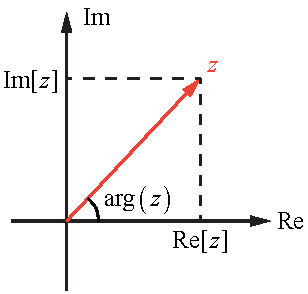
\includegraphics[width=4.7cm]{./figures/CplxNo_1.pdf}
\caption{复平面与复数} \label{CplxNo_fig1}
\end{figure}

由此可以看到, 复数跟二维平面上的几何矢量\upref{GVec}是十分相似的. 如\autoref{CplxNo_fig1}, 一个复数可以看做\textbf{复平面}上的一个点(或矢量), 该矢量在复平面的\textbf{实轴}和\textbf{虚轴}方向的分量分别等于其实部和虚部. 复数的\textbf{模}定义为对应矢量的模, 即
\begin{equation}
\abs{z} = \sqrt{\Re[z]^2 + \Im[z]^2}
\end{equation}
另外我们把矢量与实轴的夹角称为\textbf{幅角}, 记为 $\arg(z)$. 我们可以通过 $\Arctan$ 函数(\autoref{Arctan_eq1}~\upref{Arctan})计算幅角
\begin{equation}
\arg(z) = \Arctan(\Im[z], \Re[z])
\qquad (\arg z \in (-\pi, \pi])
\end{equation}
也可以通过模和幅角来计算实部与虚部
\begin{equation}
\Re[z] = \abs{z}\cos(\arg z) \qquad \Im[z] = \abs{z}\sin(\arg z)
\end{equation}
在“指数函数(复数)\upref{CExp}” 中我们将看到, 任意复数也可以通过欧拉公式表示为以下形式
\begin{equation}
z = A(\cos\theta + \I\sin\theta) = A\E^{\I\theta}
\end{equation}
其中 $A = \abs{z}$, $\theta = \arg z$.

\subsection{基本运算}
\subsubsection{共轭}
一个复数的共轭等于与其实部相同,虚部相反的复数\footnote{一些教材也使用 $\bar z$ 表示 $z$ 的共轭.}
\begin{equation}\label{CplxNo_eq6}
z\Cj = \Re[z] - \I\, \Im[z]
\end{equation}
所以共轭运算不改变复数的模, 但将其幅角变为相反数. 在复平面上, 这相当于把一个点关于 $x$ 轴取镜像对称.

\subsubsection{加和减}
复数的加减就是把两个复数的实部与虚部分别相加减(为了书写方便, 这里把复数 $z_i$ 的实部虚部记为 $x_i, y_i$)
\begin{equation}
z_1 \pm z_2 = (x_1 \pm x_2) + \I (y_1 \pm y_2)
\end{equation}
在复平面上, 这相当于把两个复数对应的矢量进行矢量相加减. 显然, 复数的加法满足交换律, 分配律和结合律.

特殊地, 将一个复数与其复共轭加减可得
\begin{equation}\label{CplxNo_eq3}
\Re[z] = \frac12 (z + z\Cj) \qquad
\Im[z] = \frac12 (z - z\Cj)
\end{equation}

\subsubsection{乘法}
两个复数相乘定义为(注意\autoref{CplxNo_eq1} 是该定义的一种特殊情况)
\begin{equation}
z_1z_2 = (x_1 + \I y_1)(x_2 + \I y_2) = (x_1 x_2 - y_1 y_2) + \I (x_1 y_2 + x_2 y_1)
\end{equation}

可以证明, 乘积的模等于两复数模之积, 乘积的幅角等于两复数的幅角之和, 即
\begin{equation}
\abs{z_1 z_2} = \abs{z_1}\abs{z_2}
\end{equation}
\begin{equation}
\arg(z_1 z_2) = \arg(z_1) + \arg(z_2)
\end{equation}
证明: 令 $A_i = \abs{z_i}$, $\theta_i = \arg z_i$, 则
\begin{equation}\ali{
z_1 z_2 &= (A_1 \cos\theta_1 + \I A_1 \sin\theta_1)(A_2 \cos\theta_2 + \I A_2 \sin\theta_2)\\
&= A_1 A_2 (\cos\theta_1\cos\theta_2 - \sin\theta_1\sin\theta_2) + \I A_1 A_2 (\cos\theta_1\sin\theta_2 + \cos\theta_2\sin\theta_1)\\
&= A_1 A_2 [\cos(\theta_1 + \theta_2) + \I \sin(\theta_1 + \theta_2)]
}\end{equation}
其中最后一步用到了两角和公式(\autoref{TriEqv_eq1}~\upref{TriEqv}). 容易看出, 最后得到的是一个模为 $A_1 A_2$, 幅角为 $\theta_1 + \theta_2$ 的复数. 证毕.

不难证明复数的乘法满足\textbf{交换律}和\textbf{结合律}. 容易证明,一个复数模的平方可以用它和复共轭的乘积表示.
\begin{equation}\label{CplxNo_eq2}
x^2 + y^2 = \abs{z}^2 = z z\Cj
\end{equation}

\subsubsection{除法}
和实数一样, 复数的除法也可以根据乘法定义. 令 $z_1 = z z_2$, 则两个复数相除可以记为
\begin{equation}
z = \frac{z_1}{z_2} = \frac{x_1 + \I y_1}{x_2 + \I y_2}
\end{equation}
但我们希望可以将结果的实部与虚部分开, 于是我们可以在分式上下同时乘以 $z_2\Cj$, 即 $z_1 z_2\Cj  = z z_2 z_2\Cj$, 或
\begin{equation}
z = \frac{z_1 z_2\Cj}{z_2 z_2\Cj}
= \frac{(x_1 + \I y_1)(x_2 - \I y_2)}{(x_2 + \I y_2)(x_2 - \I y_2)}
= \frac{x_1 x_2 + y_1 y_2}{x_2^2 + y_2^2} + \I \frac{x_2 y_1 - x_1 y_2}{x_2^2 + y_2^2}
\end{equation}
这个步骤叫做\textbf{分母有理化}.

与乘法同理, 两个复数相除相当于把它们的模相除, 幅角相减, 即
\begin{equation}
\abs{z_1/z_2} = \abs{z_1}/\abs{z_2}
\end{equation}
\begin{equation}
\arg(z_1/z_2) = \arg(z_1) - \arg(z_2)
\end{equation}

根据定义易证
\begin{theorem}{}\label{CplxNo_the1}
两个复数进行任意次加减乘除后再取共轭, 等于它们分别取共轭后再进行运算.
\end{theorem}
例如
\begin{equation}
\frac{2 z_1 z_2}{(z_3 + z_4)^2} = \frac{2 z_1^* z_2^*}{(z_3^* + z_4^*)^2}
\end{equation}

根据\autoref{CplxNo_eq2}, \autoref{CplxNo_eq3} 和\autoref{CplxNo_the1} 易得
\begin{equation}
\abs{z_1 + z_2}^2 = \abs{z_1}^2 + \abs{z_2}^2 + z_1^* z_2 + z_2^* z_1 = \abs{z_1}^2 + \abs{z_2}^2 + 2\Re[z_1^* z_2]
\end{equation}
在复平面中, 该式可以表示余弦定理, 即计算两矢量之和的模.
